\documentclass[prl,preprint]{revtex4-1}
%\documentclass[12pt]{article}

\usepackage{amsmath}
\usepackage{amsfonts}

\usepackage{graphicx}
\usepackage{subcaption}

\begin{document}

The problem setting:\\
 We have a simulation of the dynamical system that is governed basically by a single parameter,­ the rate of switching.
 %
 Depending of the value of this parameter, this system dynamics range between heat equation dynamics and wave equation dynamics. 
 %
 In the heat equation dynamics, the initial conditions play very little role and the system dynamics over time are dominant. 
 %
 In the wave equation dynamics, the initial conditions play a significant role and the dynamics over time are less important.


Contribution: 
\begin{enumerate}
\item We demonstrate that an essential component of our analysis is working with the right observers (histograms/ensumble rather than a single position of a particle) and with the right metric between those observers (EMD).
%
\item We demonstrate that we recover the right factors that control the dynamical system, depending on the mode (In heat eq. mode ­ first recover the temporal dynamics, second the initial conditions; In wave eq. mode ­ first recover the initial conditions, second the temporal dynamics). In particular, these two components have a completely different ``nature". For example, in this case, one parameter (initial condition) is governing the entire trajectory and the other parameter (dynamics) is governing the ``step­--by­--step" time evolution (within each trajectory).
\end{enumerate}

\section{Introduction}

In dynamical systems, it is often essential to detect changes in the characteristic behavior of a system.
%
Methods such as bifurcation analysis, etc., have been developed with such problems in mind. 

We will demonstrate how we can use data mining techniques (diffusion maps \cite{...}) to {\em automatically} detect changes in a system's behavior.
%
We will illustrate our dynamics through a model problem arising in studies of cellular chemotaxis \cite{...}.
%
In our methods, it will be esseintial 


\section{Problem formualtion}

\subsection{Chemotaxis ``story''} 

We look at a stochastic velocity jump process that arises in models of chemotaxis \cite{othmer2000diffusion}.
%
Chemotaxis is movement in cells (such as bacteria) that is regulated by extracellular censed signals.
%
Cells must move to accomplish tasks such as finding food and navigating away from toxins, and this movement is thought to be directed by such extracellular signals.
%
Biologists are interested in the dynamics of dispersal of cells, and several models have been proposed \cite{othmer1988models, codling2008random}.
%
We will look at a velocty jump process as a model of these dynamics.
%
In such models, each cell is initialized with a position and a velocity, and the dynamics of each cell are goverened by a stochastic process.
%
In a velocity jump process, at random times, cells will ``turn around'' and switch their velocity (in biology, this turning is thought to be driven by extracellular signals such as food or toxins). 
%
We will analyze the dynamics of collections of such cells/particles. 

\subsection{Stochastic particles}

We have a collection of $N$ particles, each of which has a position and velocity. 
%
Let $x_i(t)$ and $v_i(t)$ denote the position and velocity, respectively, of particle $i$ at time $t$.
%
The velocity of each particle is either $\pm s$, where $s$ is the speed. 
%
We initialize the particles such that
\begin{eqnarray}
x_i(0) & = 0 \\
\mathbb{P} \{ v_i(0) = +s \} & = p
\end{eqnarray}
where $p$ is some probability.
%
The velocity of each particle randomly switches between $\pm s$ following an (independent) Poisson process with rate $\lambda$.
%
Note that each particle has its own ``clock" (Poisson process).

\subsection{Partial differential equations}

Let $X_{p, \lambda, s}(t)$ denote the vector of positions of the particles at time $t$ with initial right probability $p$, switching rate $\lambda$, and speed $s$.

Let $\rho(x, t)$ denote the probability density of the particles, and let $\rho^-(x, t)$ and $\rho^+(x, t)$ denote the probability density of the left and right moving particles, respectively.
%
It can be shown that, as $n \rightarrow \infty$, $\rho(x, t)$ obeys the following set of partial differential equations (PDEs)
\begin{eqnarray} \label{eqn:coupled_pdes}
\frac{\partial \rho^+}{\partial t} + s \frac{\partial \rho^+}{\partial x} & = -\lambda \rho^+ +\lambda \rho^- \\
\frac{\partial \rho^-}{\partial t} - s \frac{\partial \rho^-}{\partial x} & = \lambda \rho^+ -\lambda \rho^- 
\end{eqnarray}
%
Alternatively, \eqref{eqn:coupled_pdes} can be written as one, second--order PDE
\begin{equation} \label{eq:second_order_pde}
\frac{\partial^2 \rho}{\partial t^2} + 2 \lambda \frac{\partial \rho}{\partial t} = s^2 \frac{\partial ^2 \rho}{\partial x^2}
\end{equation}
%
We assume that $s^2/\lambda = D$ is constant.
%
Therefore, the dynamics are governed {\em only} by a single parameter $\lambda$.

\subsection{Asymptotic mode analysis}  \label{subsec:mode_analysis}

We will consider two regimes of simulation.
%
When $\lambda \rightarrow 0$ is small, one can see that the right-hand side of \eqref{eqn:coupled_pdes} tends to 0. 
%
Therefore, \eqref{eqn:coupled_pdes} becomes two uncoupled wave equations.
%
Alternatively, in this regime, in the limit the second order equation \eqref{eq:second_order_pde} becomes 
\[
\frac{\partial^2 \rho}{\partial t^2} = s^2 \frac{\partial ^2 \rho}{\partial x^2},
\]
i.e., the second order wave equation.

Dividing \eqref{eq:second_order_pde} by $\lambda > 0$ yields
\[
\frac{1}{\lambda} \frac{\partial^2 \rho}{\partial t^2} + 2 \frac{\partial \rho}{\partial t} = D \frac{\partial ^2 \rho}{\partial x^2}
\]
When $\lambda \rightarrow \infty$, \eqref{eq:second_order_pde} approaches the heat equation
\[
2 \frac{\partial \rho}{\partial t} = D \frac{\partial ^2 \rho}{\partial x^2}
\]
 
\section{Methods and Analysis}

\subsection{Diffusion maps}

\subsection{Earth mover's distance}

TODO: we need to pay a special attention to the implementation of the EMD. We need to make it cleat that this distance can be very efficiently implemented  and therefore it is suitable for the practical uses and algorithm that we propose here as a viable tool for dynamical system analysis.

\section{Results}
We simulate this stochastic velocity jump process for $N=1000$ particles, and $p \in [0.1, 0.9]$.
%
We simulate the process for $t \in [0, 10]$, and record the positions of each particle at uniform/equal time intervals.
%
We will consider two sets of simulations.
%
In one set, $\lambda = 1$ and $s=1$, and in the other set, $\lambda = 400$, and $s=20$.

TODO: In Fig. \ref{fig:dmaps_embed}, add representative (non degenerate and smooth) histograms in strategic embedded points.

\begin{figure}[htb]
\begin{subfigure}{0.5\textwidth}
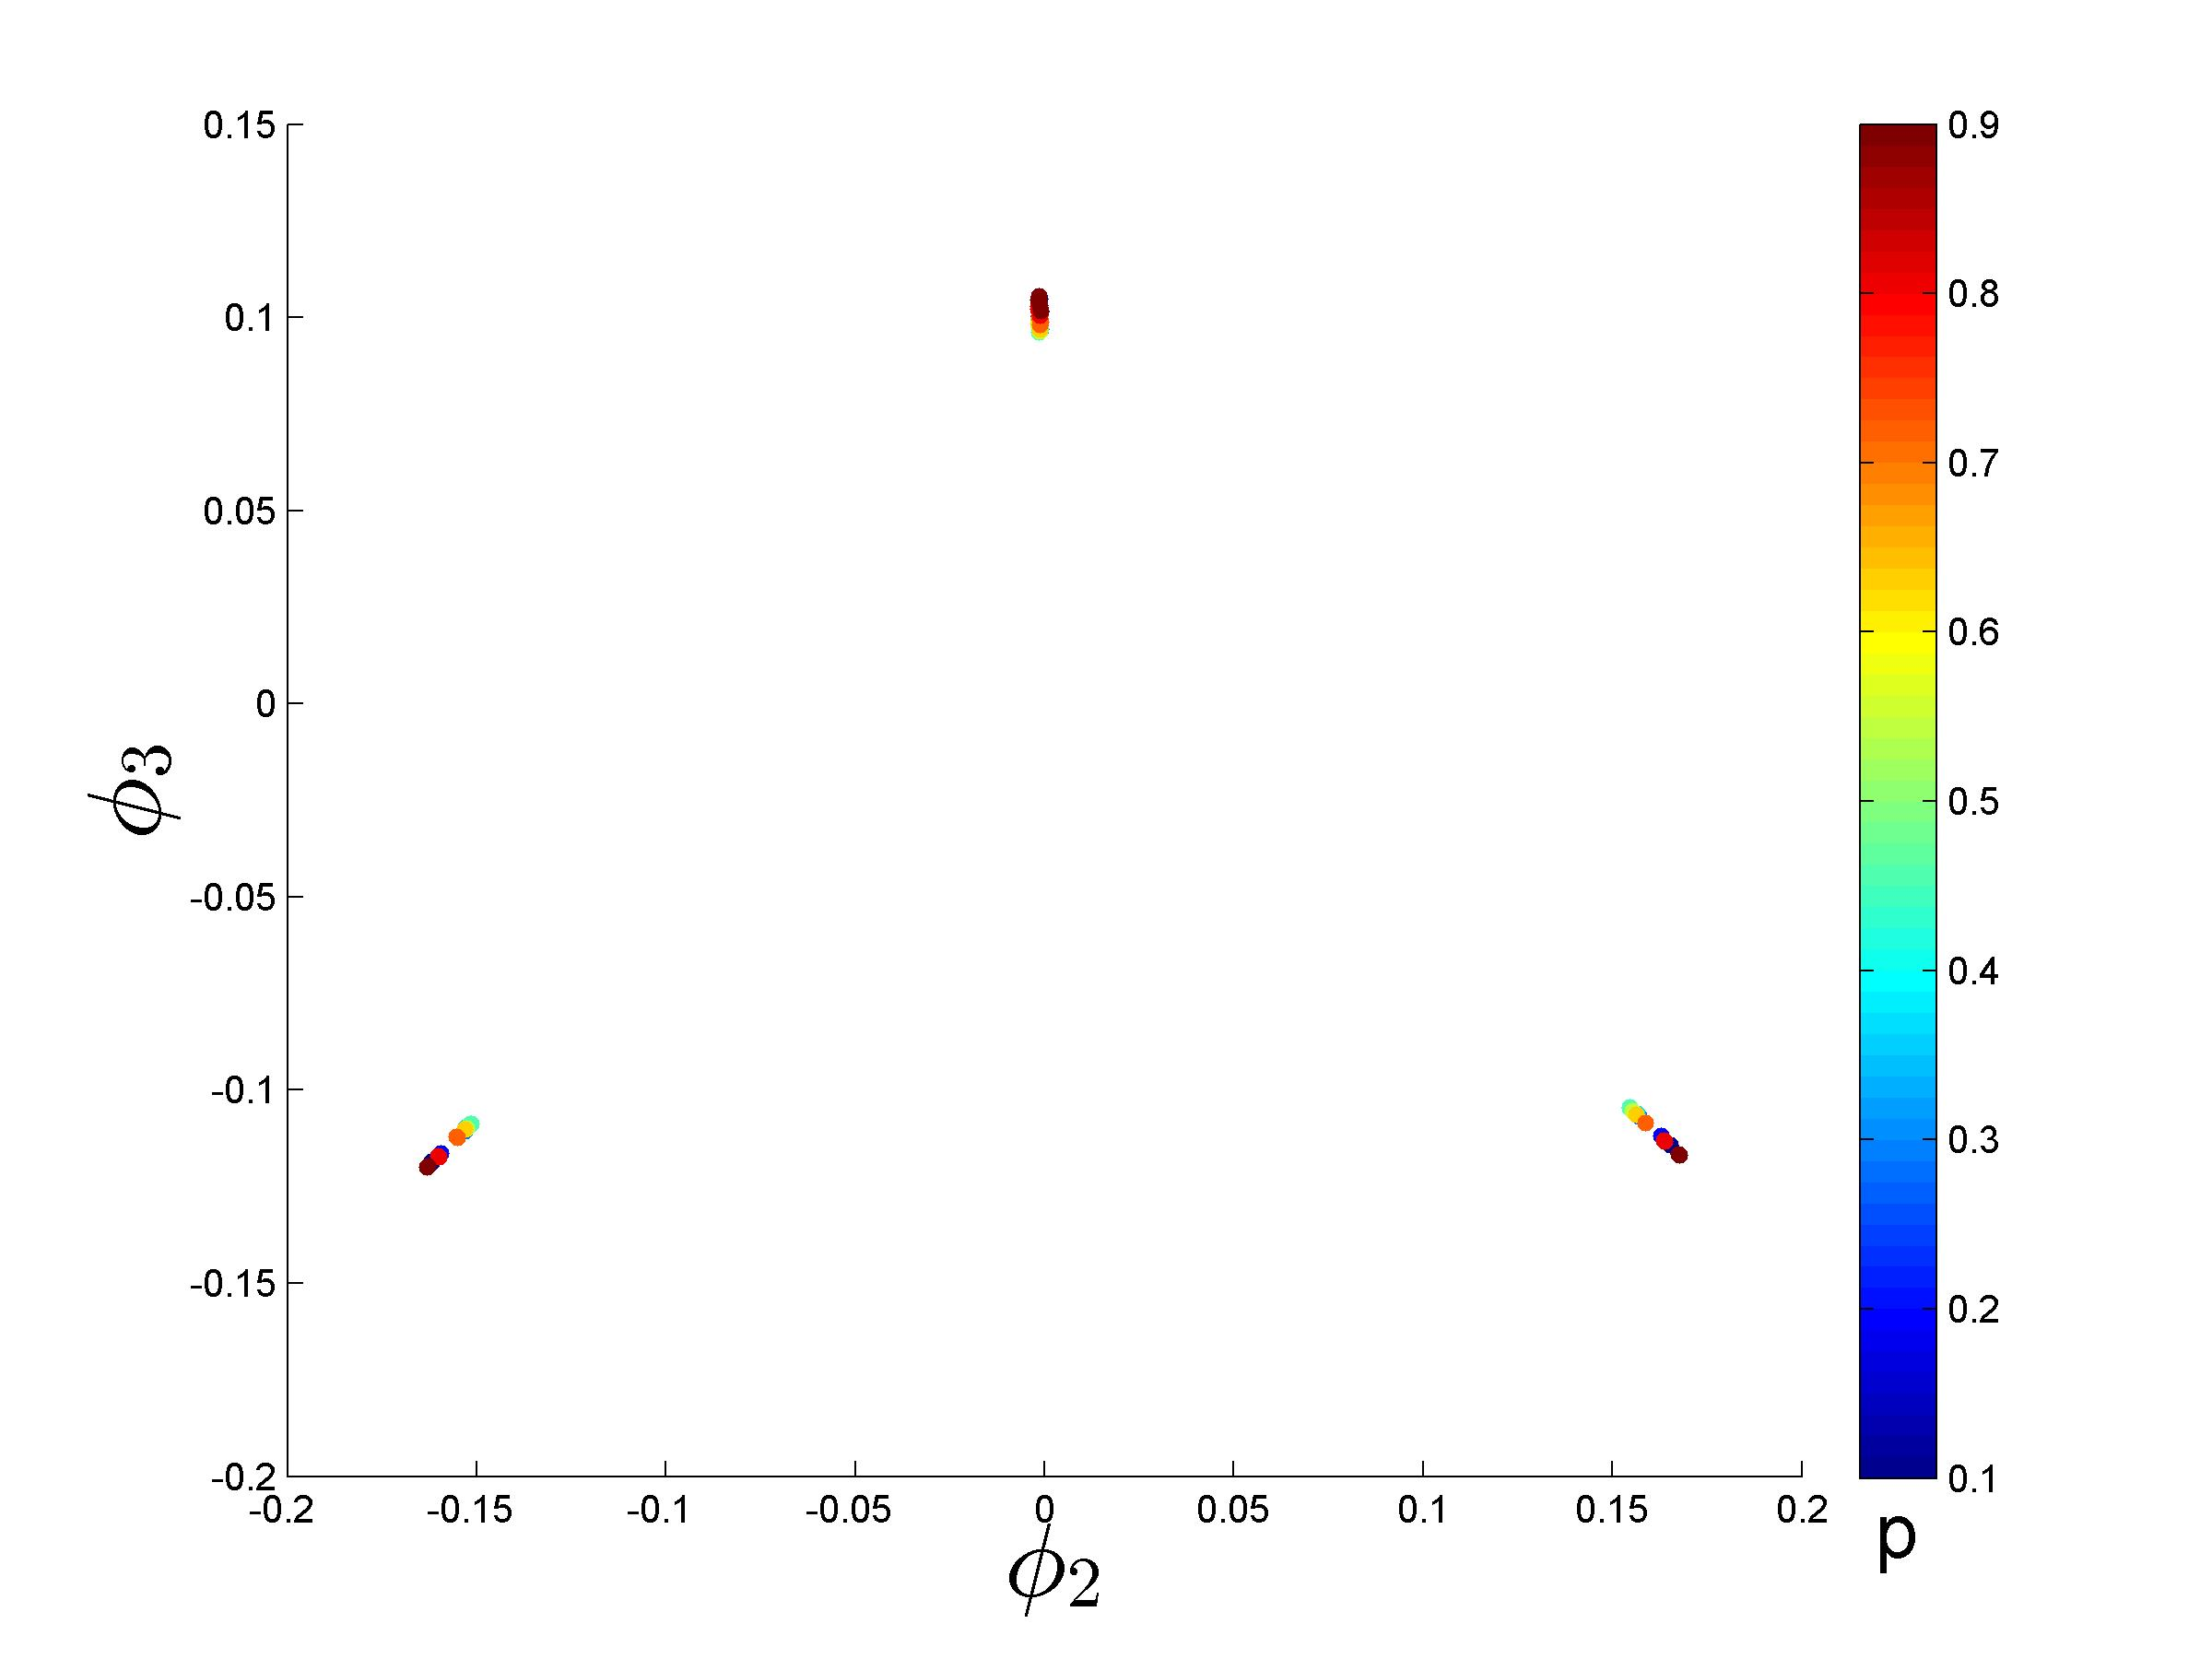
\includegraphics[width=\textwidth]{rawhist_p_1}
\caption{}
\end{subfigure}
\begin{subfigure}{0.5\textwidth}
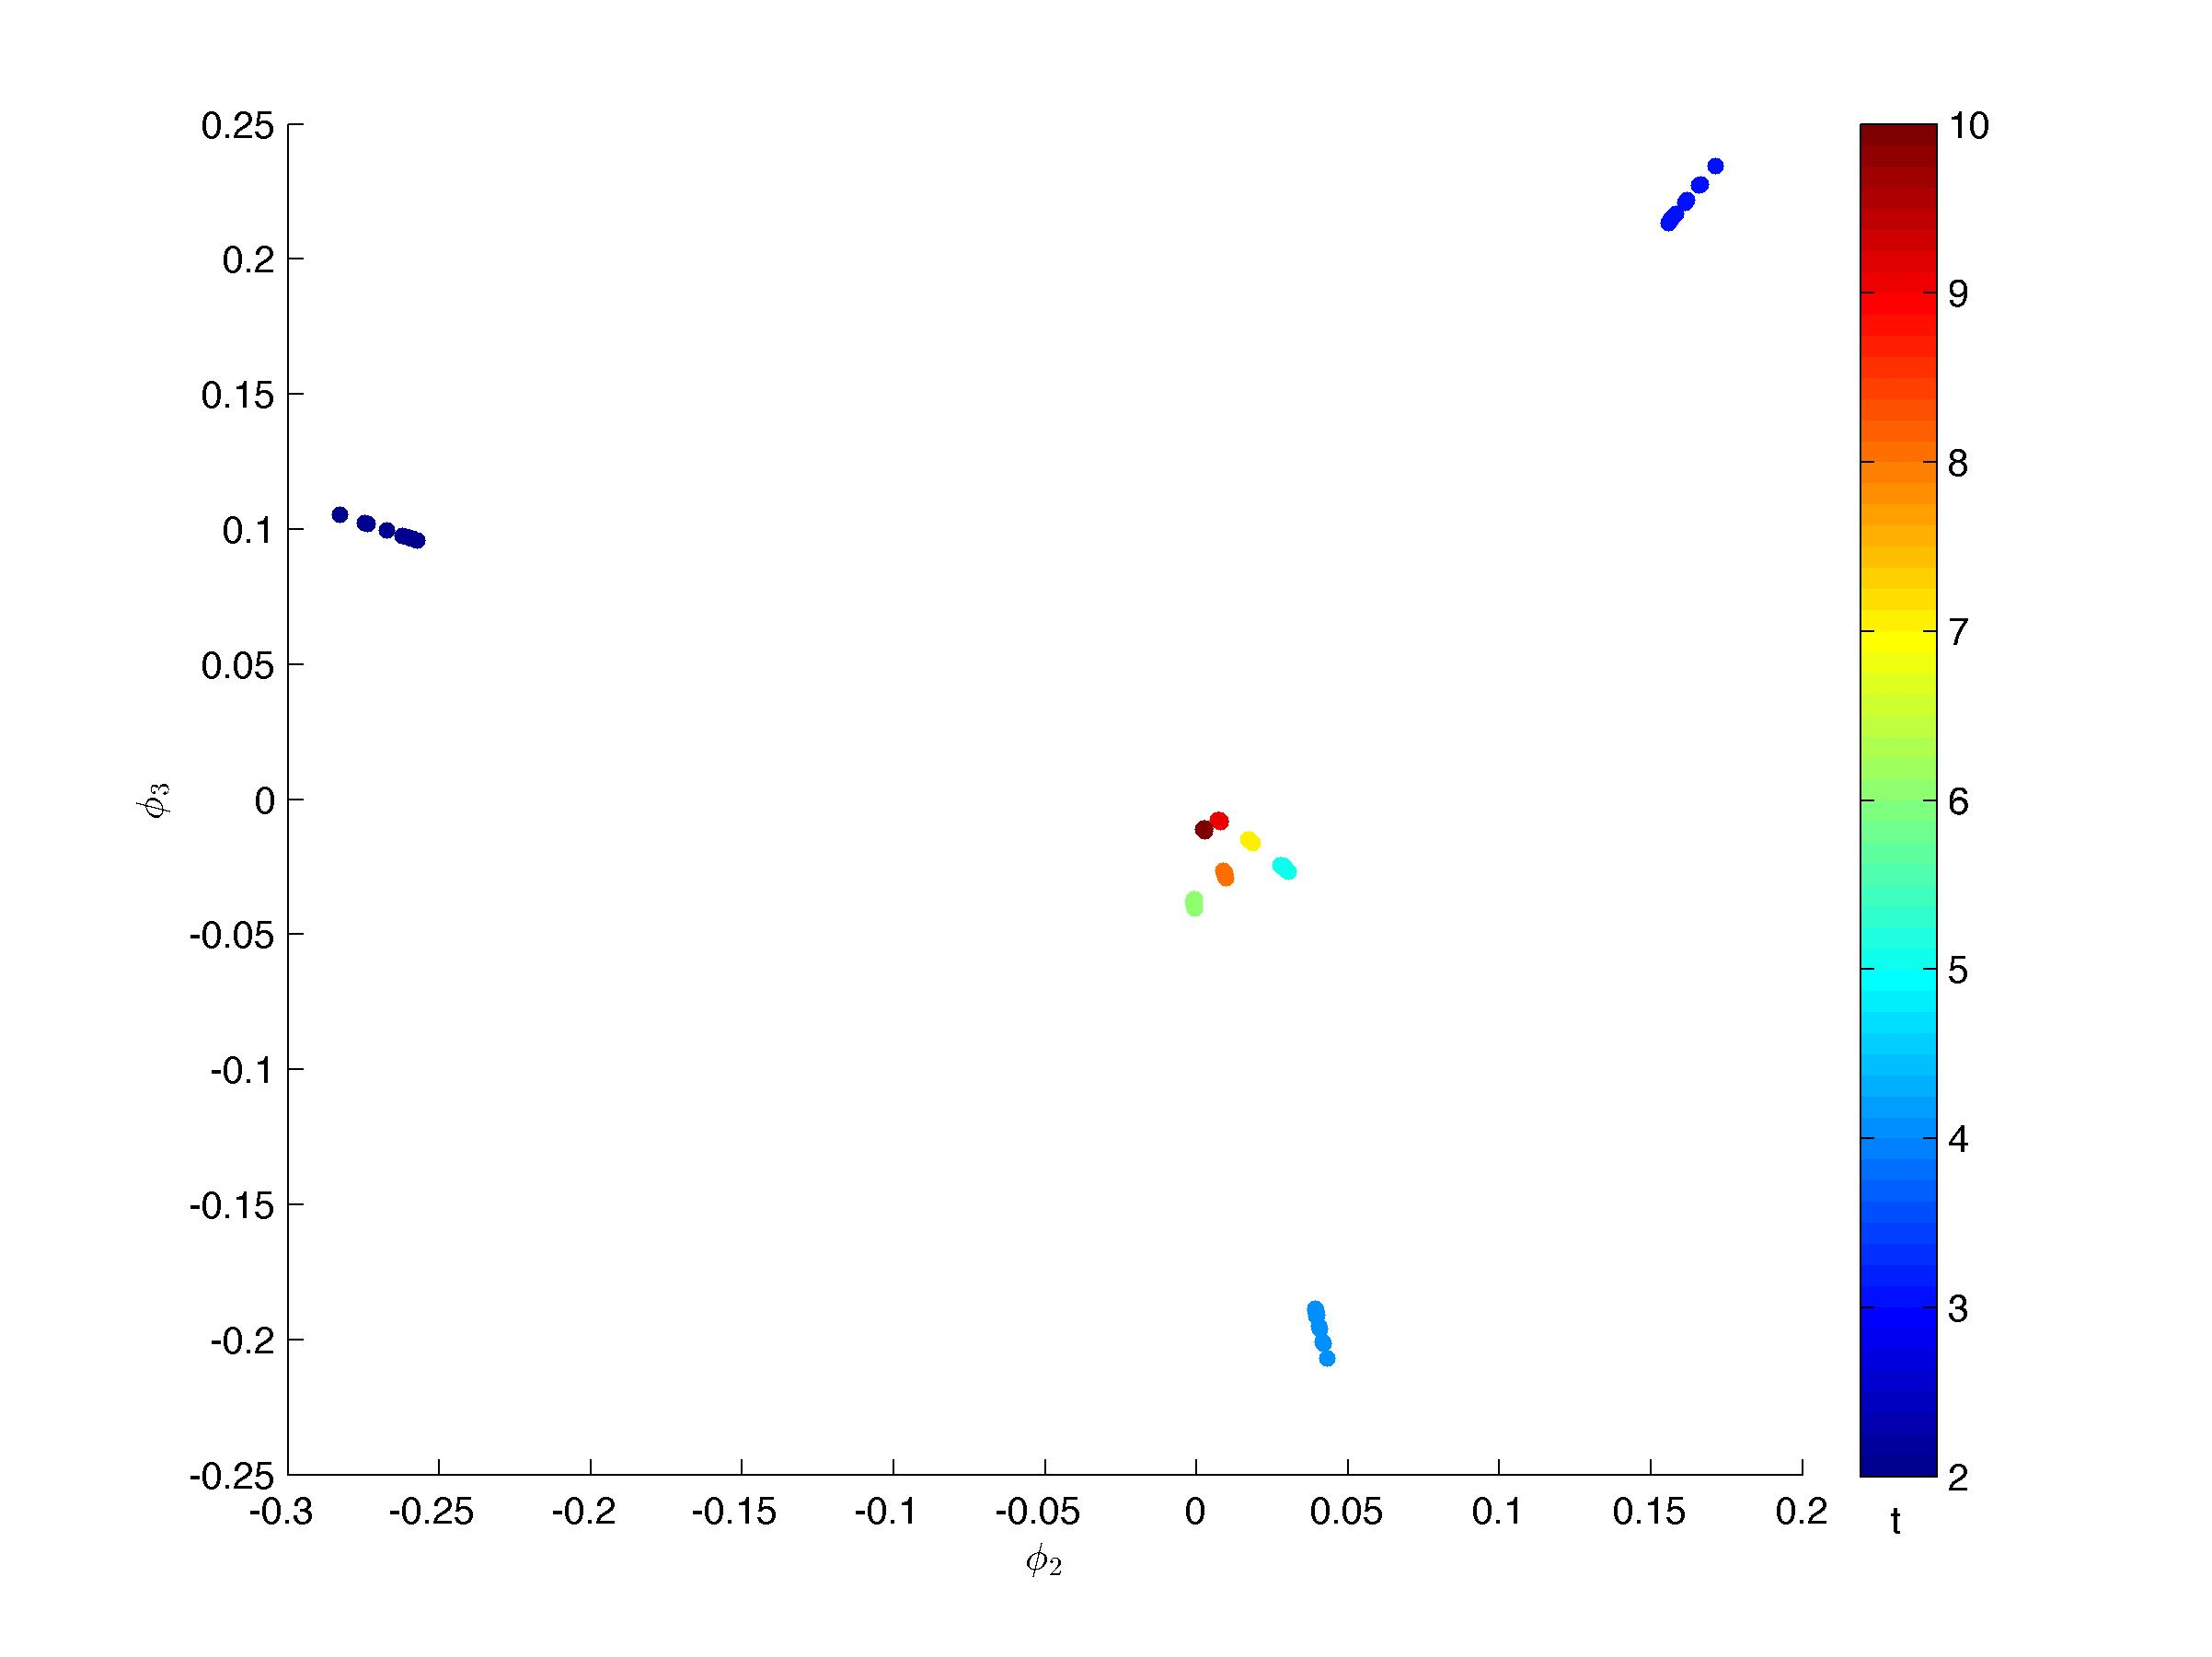
\includegraphics[width=\textwidth]{rawhist_t_1}
\caption{}
\end{subfigure}
\begin{subfigure}{0.5\textwidth}
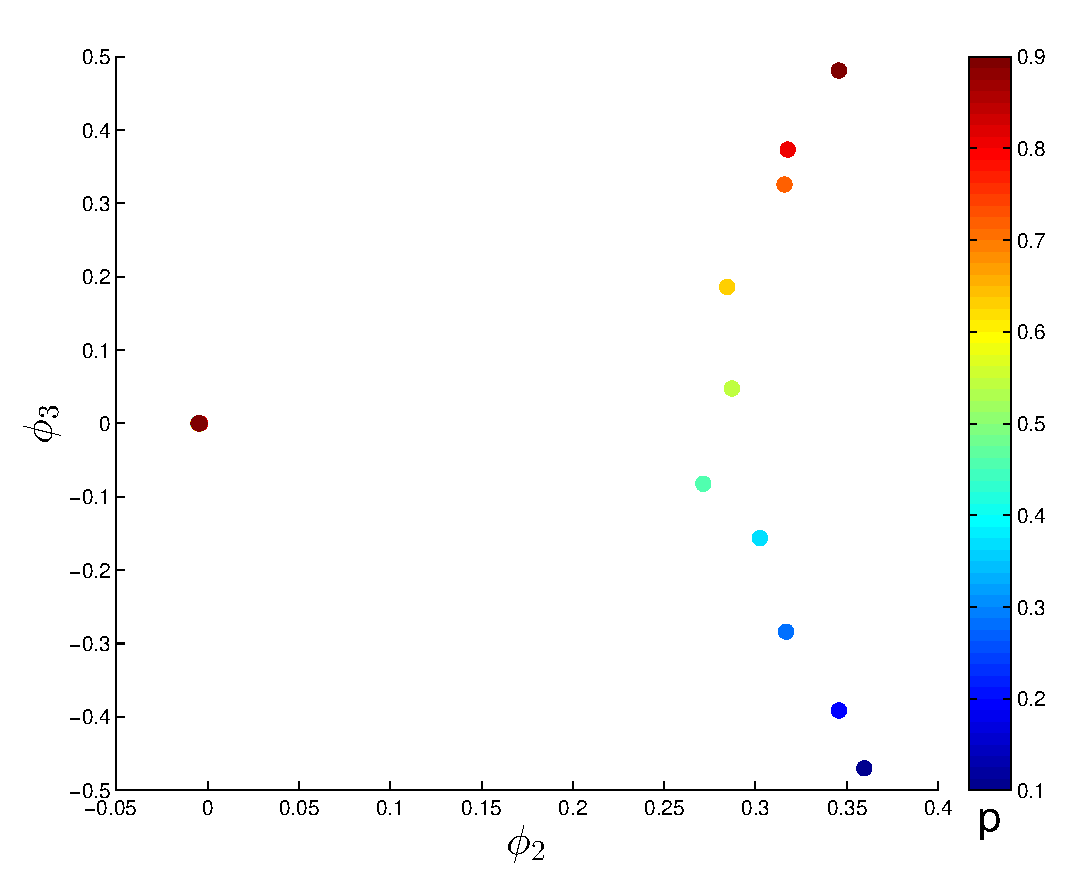
\includegraphics[width=\textwidth]{rawhist_p_400}
\caption{}
\end{subfigure}
\begin{subfigure}{0.5\textwidth}
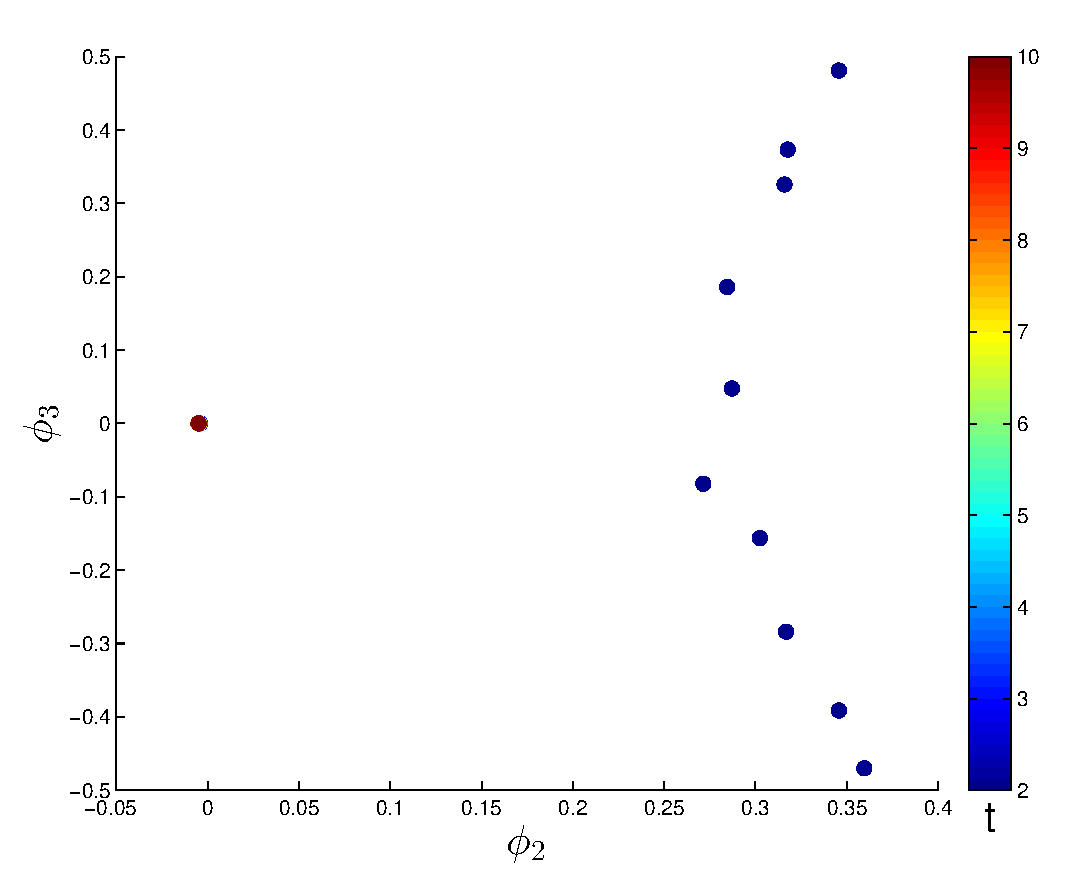
\includegraphics[width=\textwidth]{rawhist_t_400}
\caption{}
\end{subfigure}
\caption{Diffusion maps embeddings computed from simulation data of the velocity jump process with (a,b) $\lambda=1$, $s=1$, and (c,d) $\lambda=400$, $s=20$. The distances used in the diffusion maps kernel are the Euclidean distances between the histograms of particle positions. The data are colored by (a, c) $p$, the initial probability of left--moving particles, and (b, d) $t$, time. The first two diffusion maps modes do not accurately capture the important parameters in our simulations.}
\label{fig:dmaps_embed}
\end{figure}

\begin{figure}[htb]
\begin{subfigure}{0.5\textwidth}
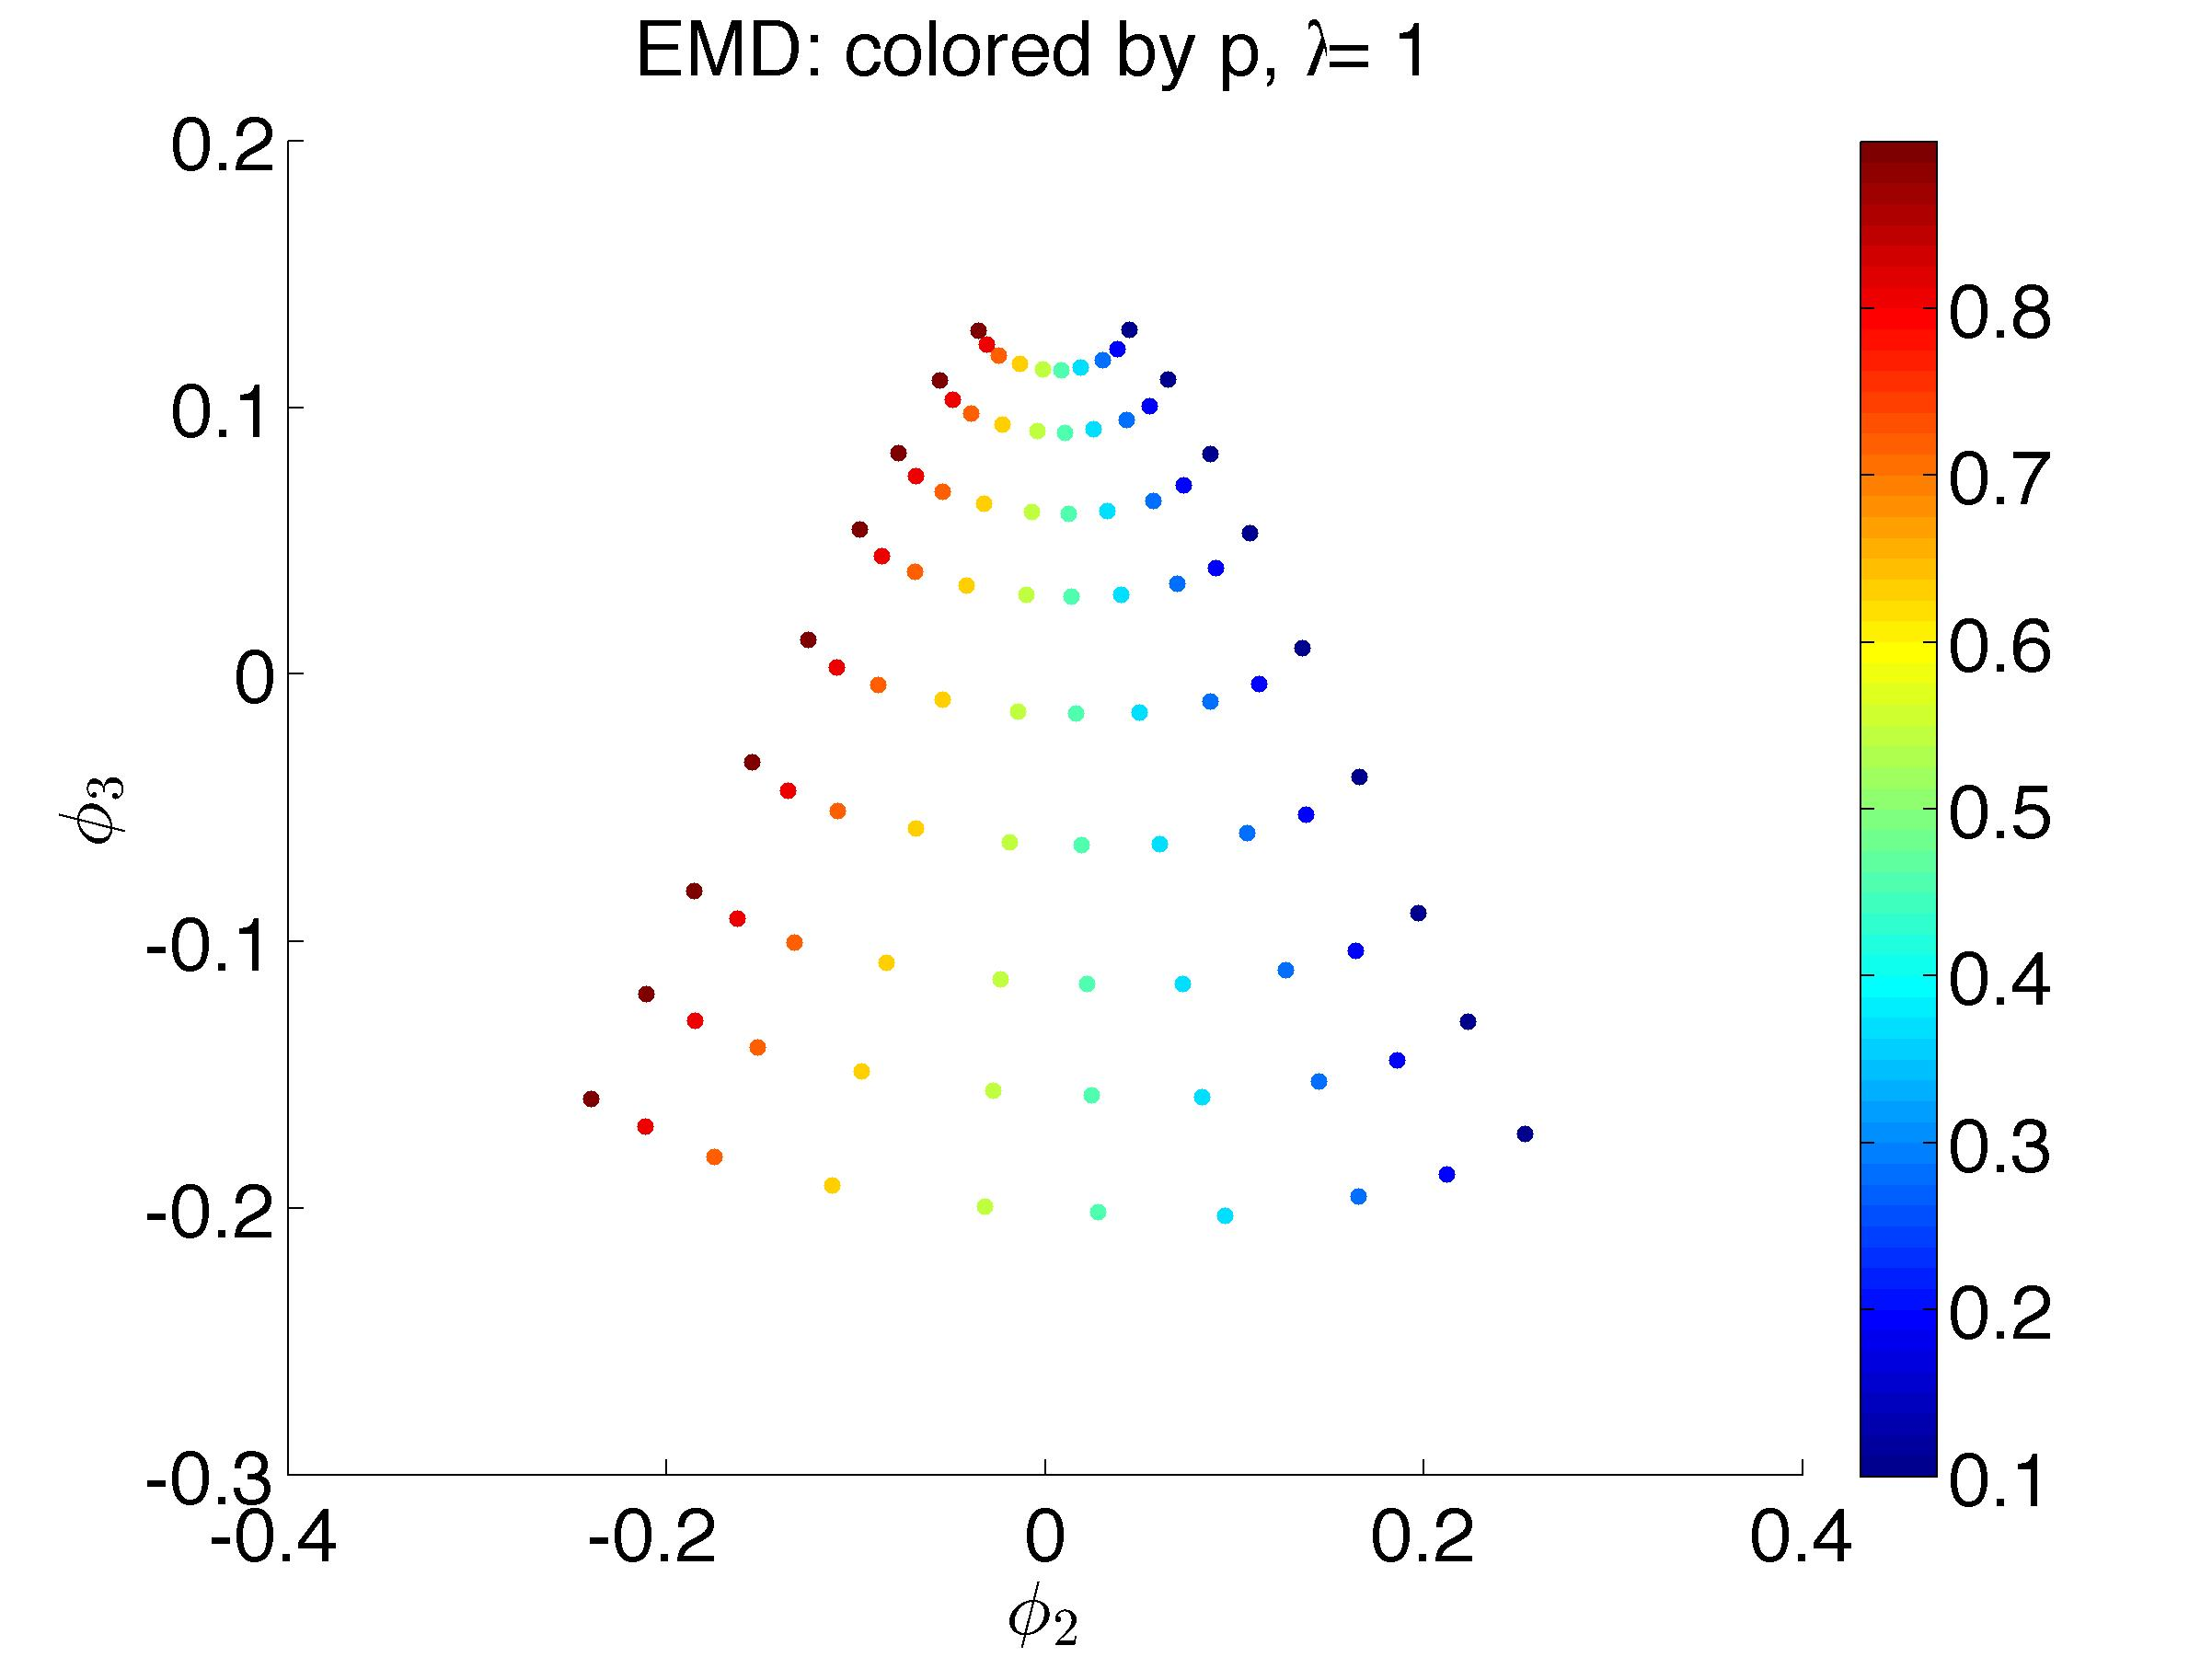
\includegraphics[width=\textwidth]{EMD_p_1}
\caption{}
\end{subfigure}
\begin{subfigure}{0.5\textwidth}
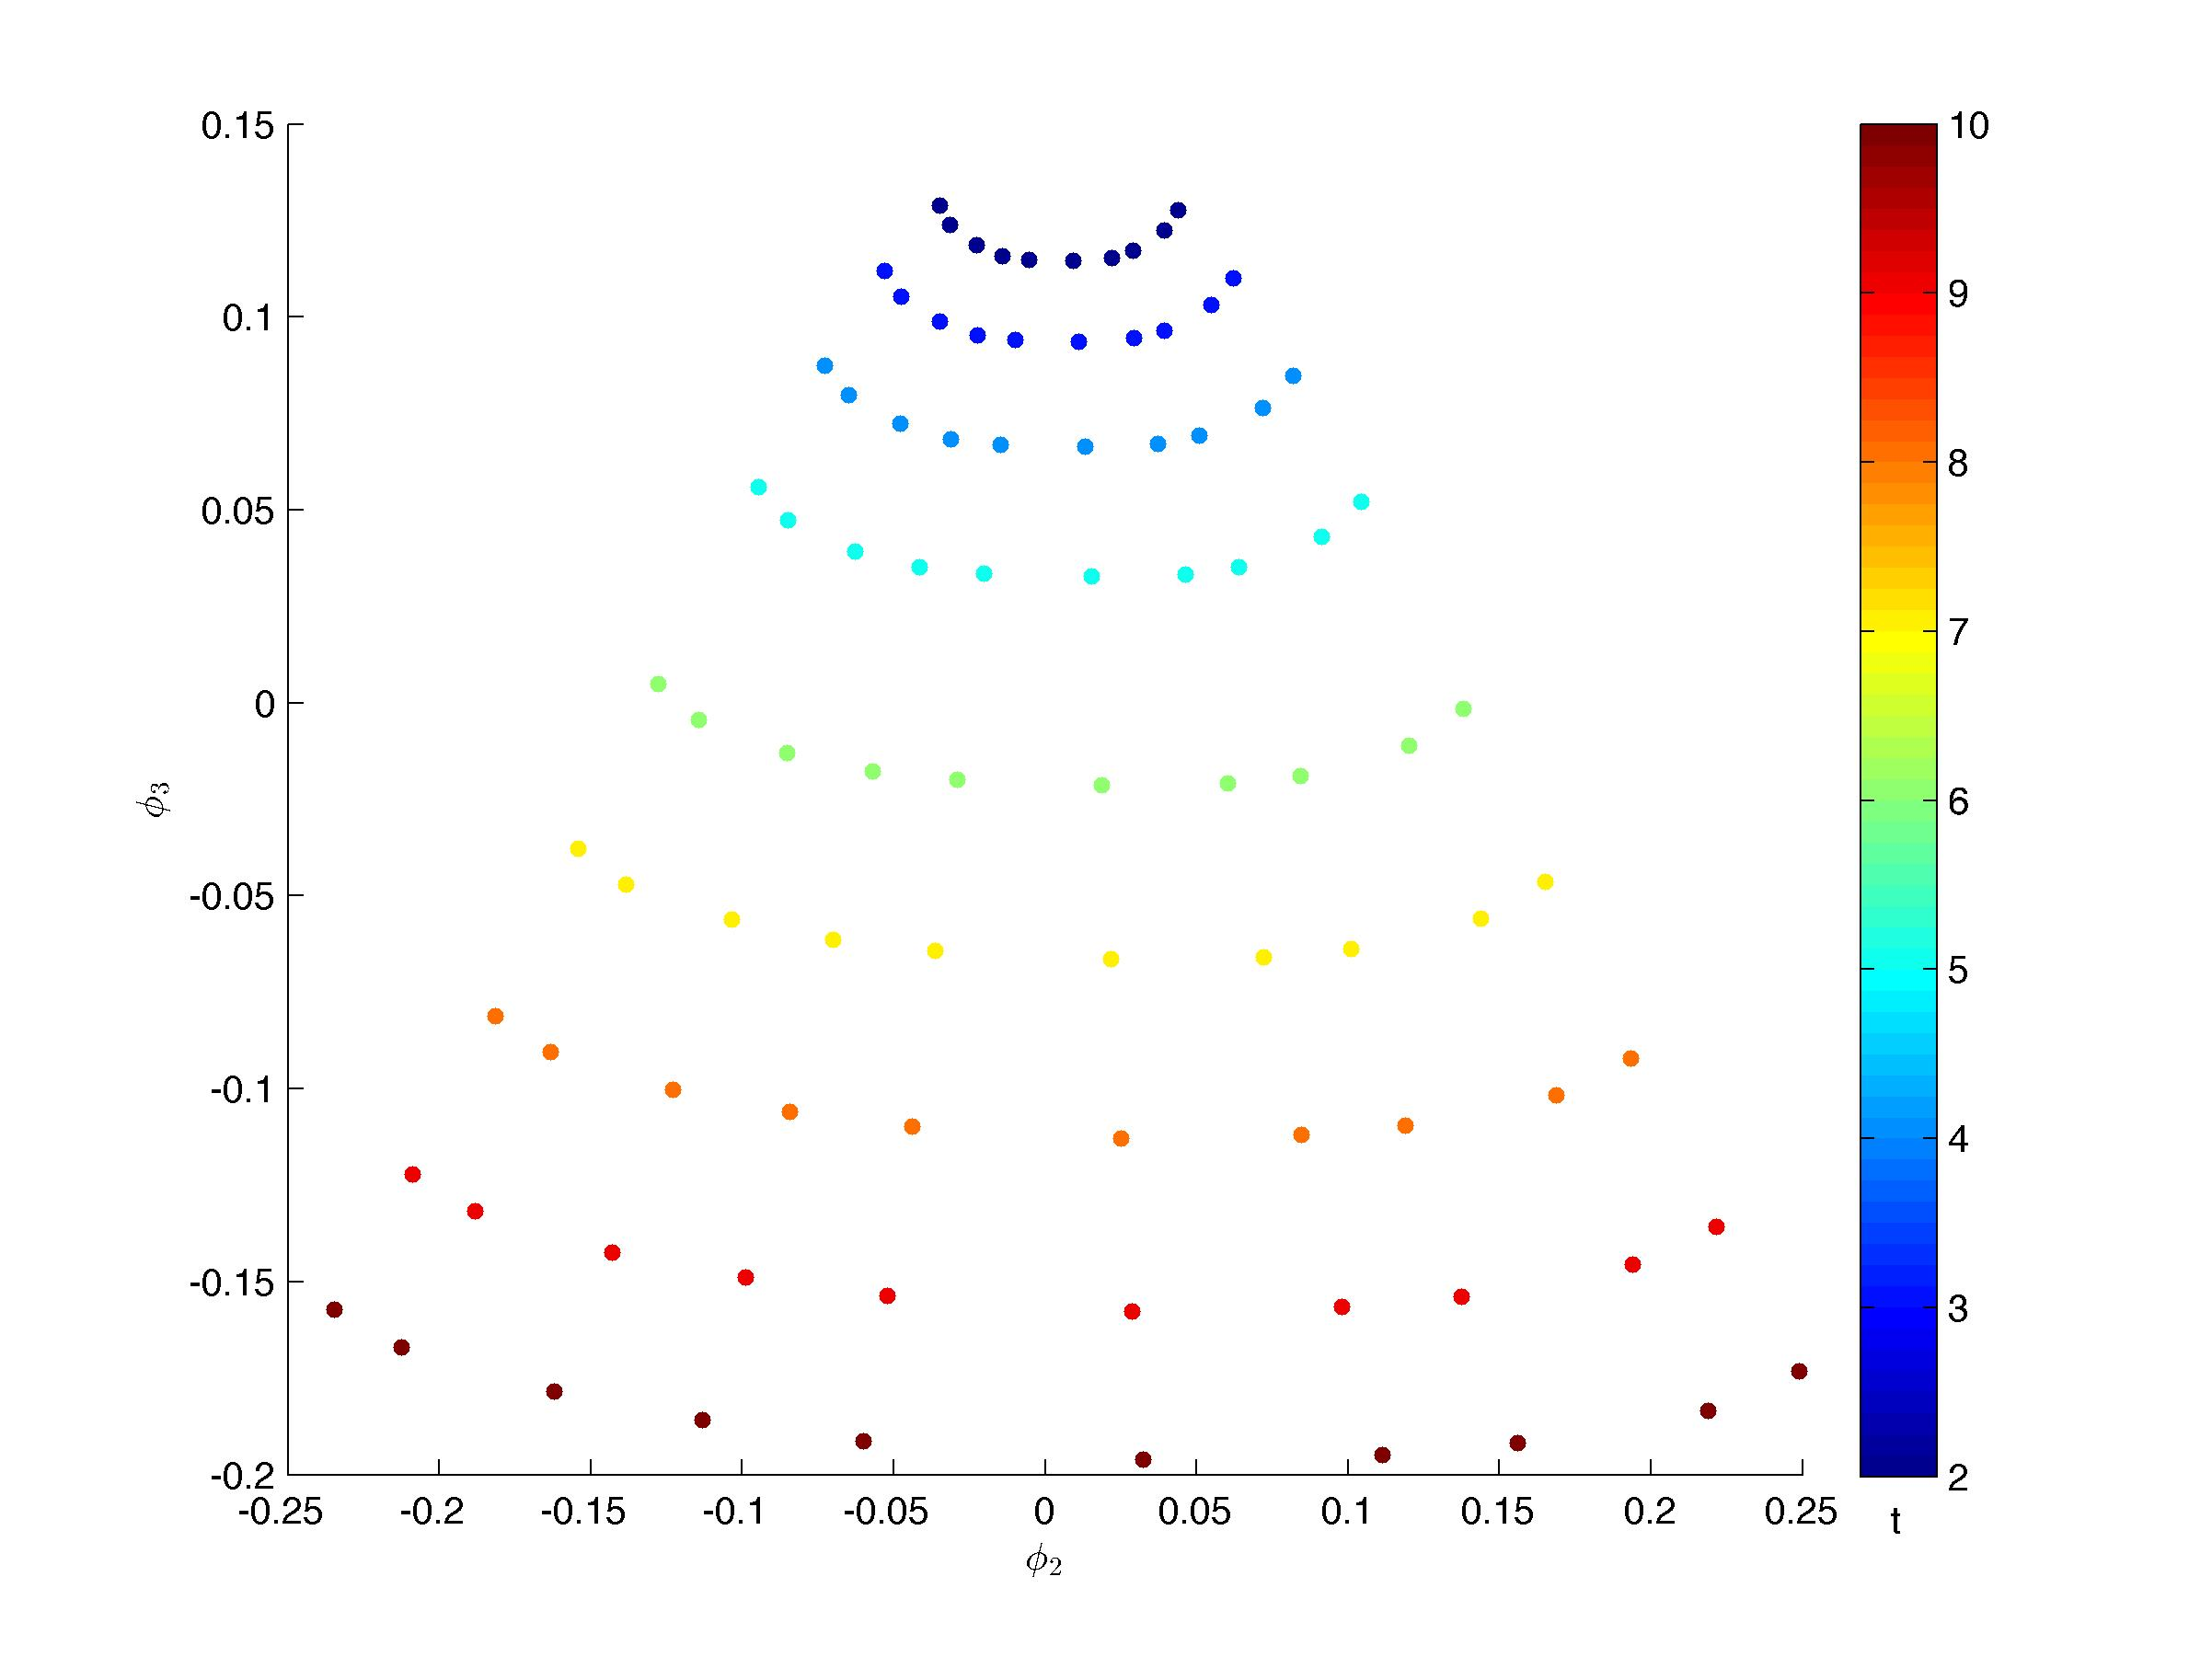
\includegraphics[width=\textwidth]{EMD_t_1}
\caption{}
\end{subfigure}
\begin{subfigure}{0.5\textwidth}
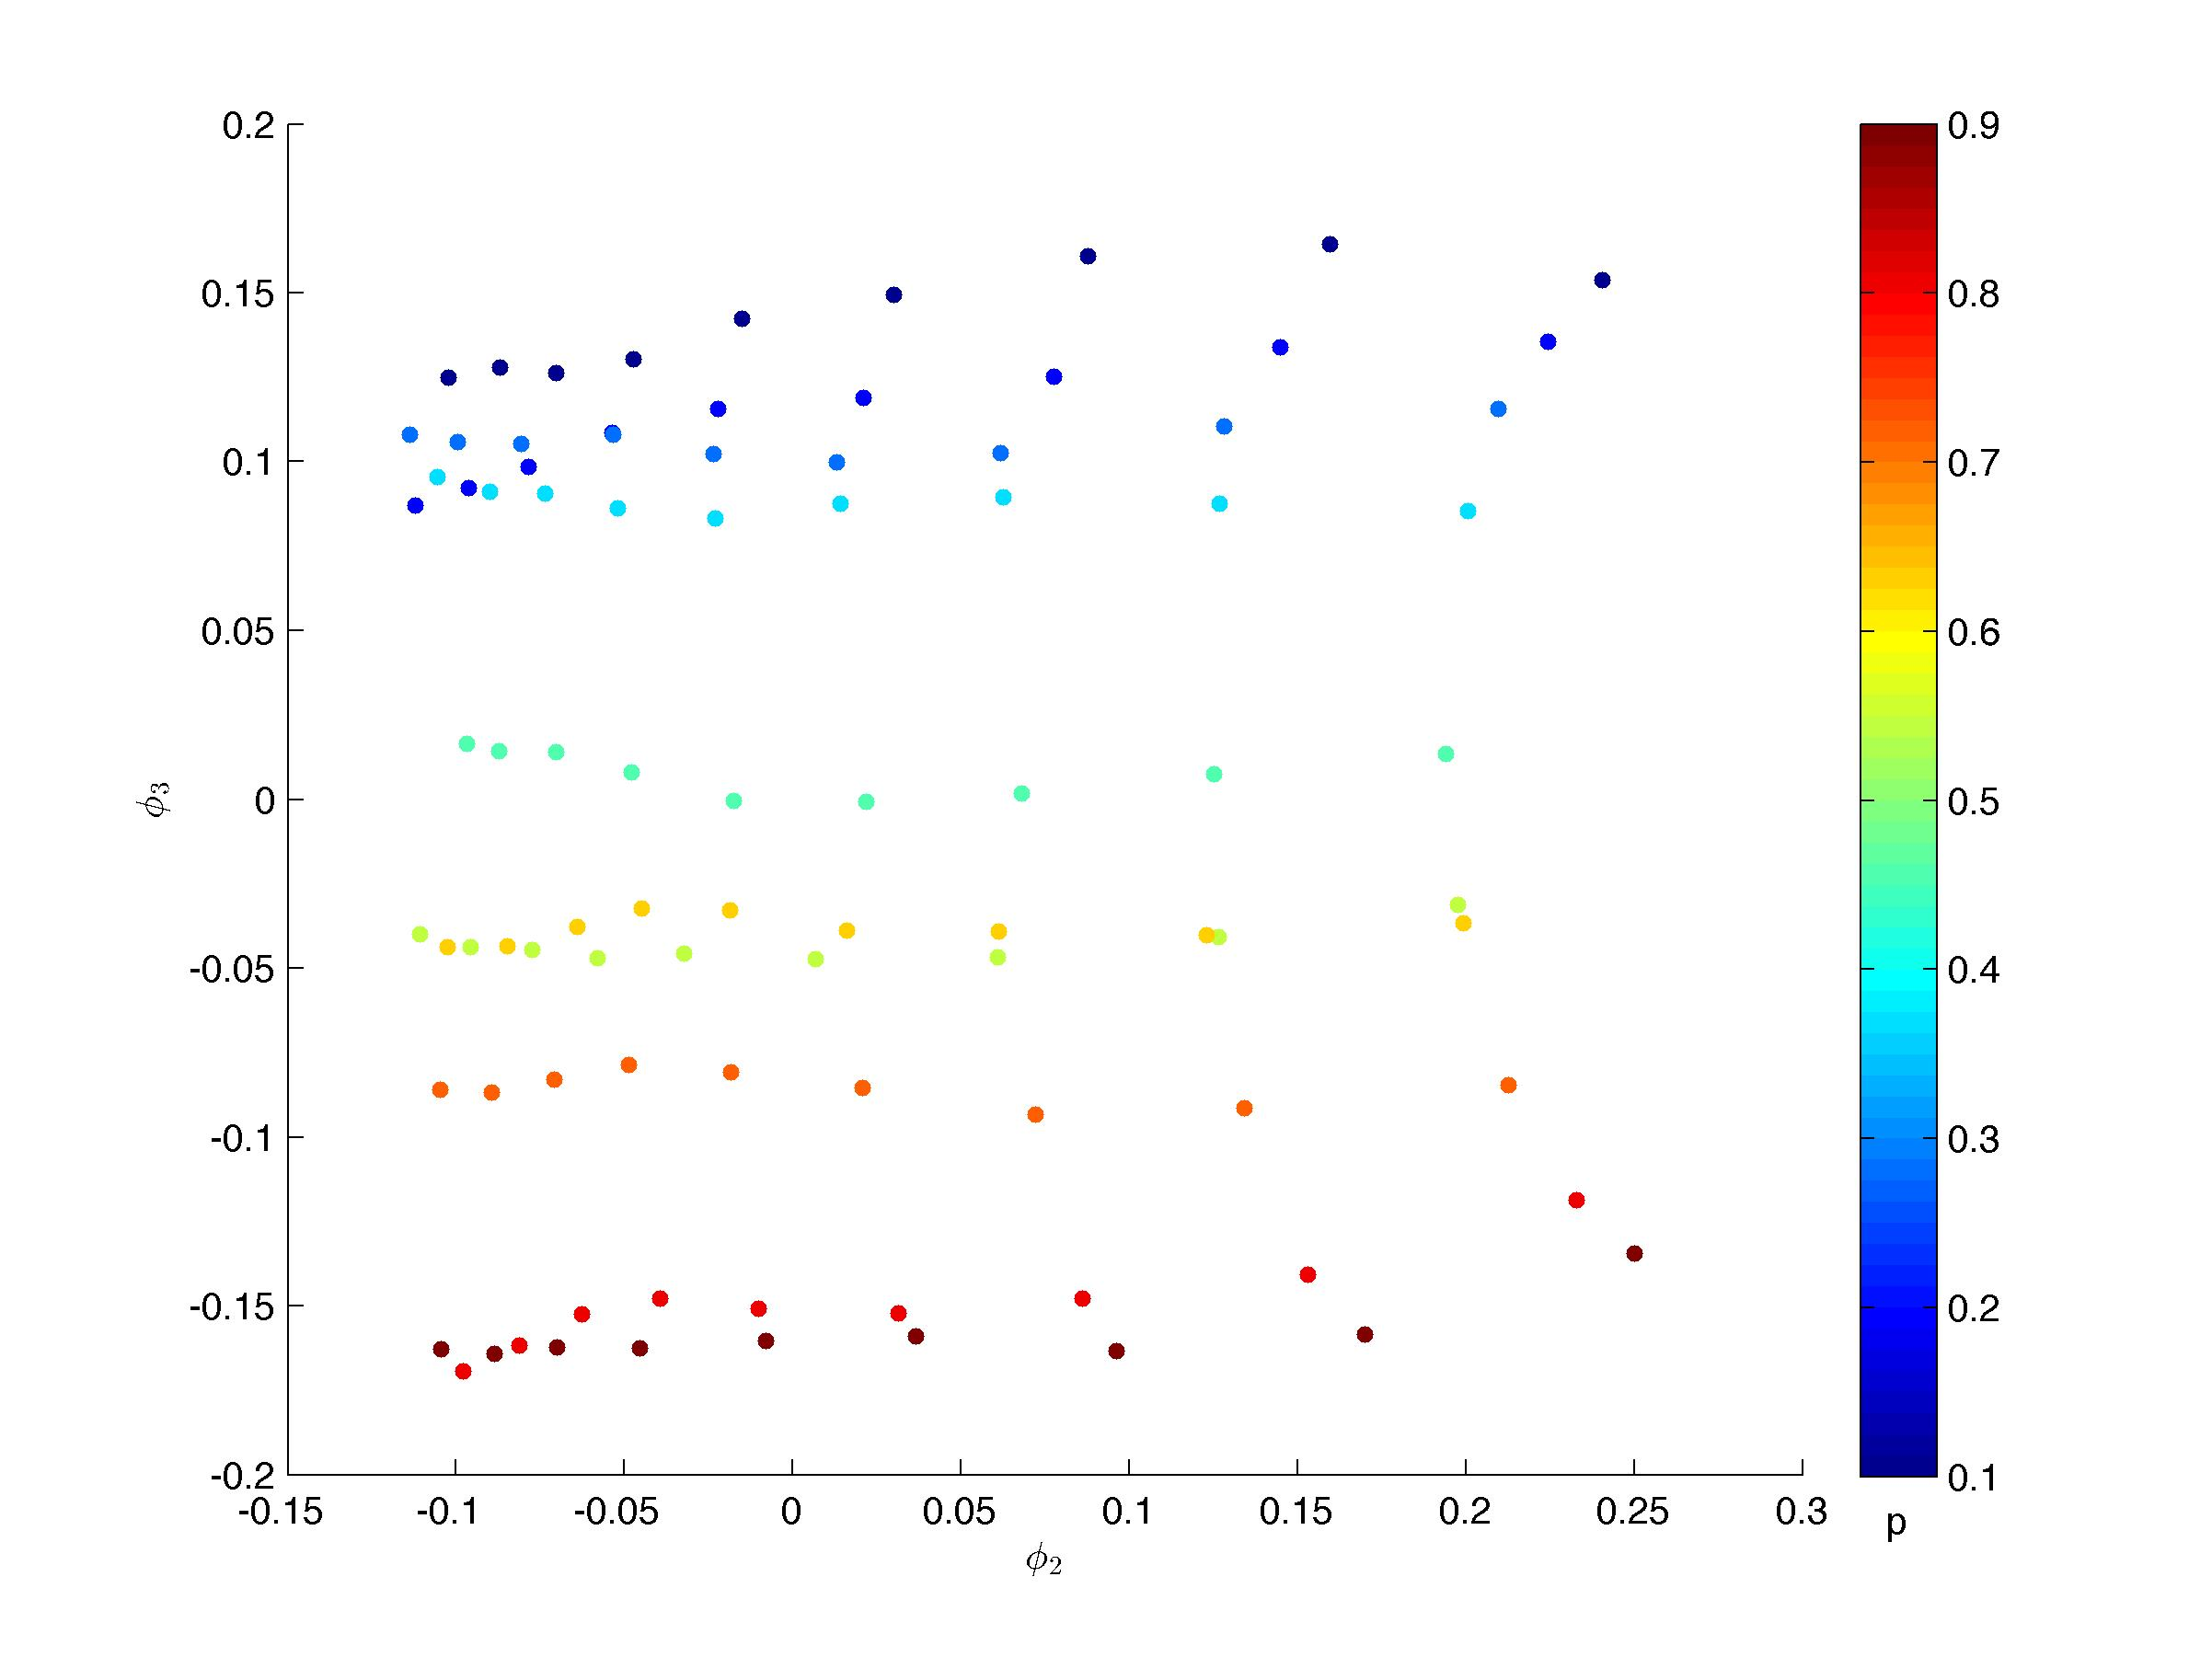
\includegraphics[width=\textwidth]{EMD_p_400}
\caption{}
\end{subfigure}
\begin{subfigure}{0.5\textwidth}
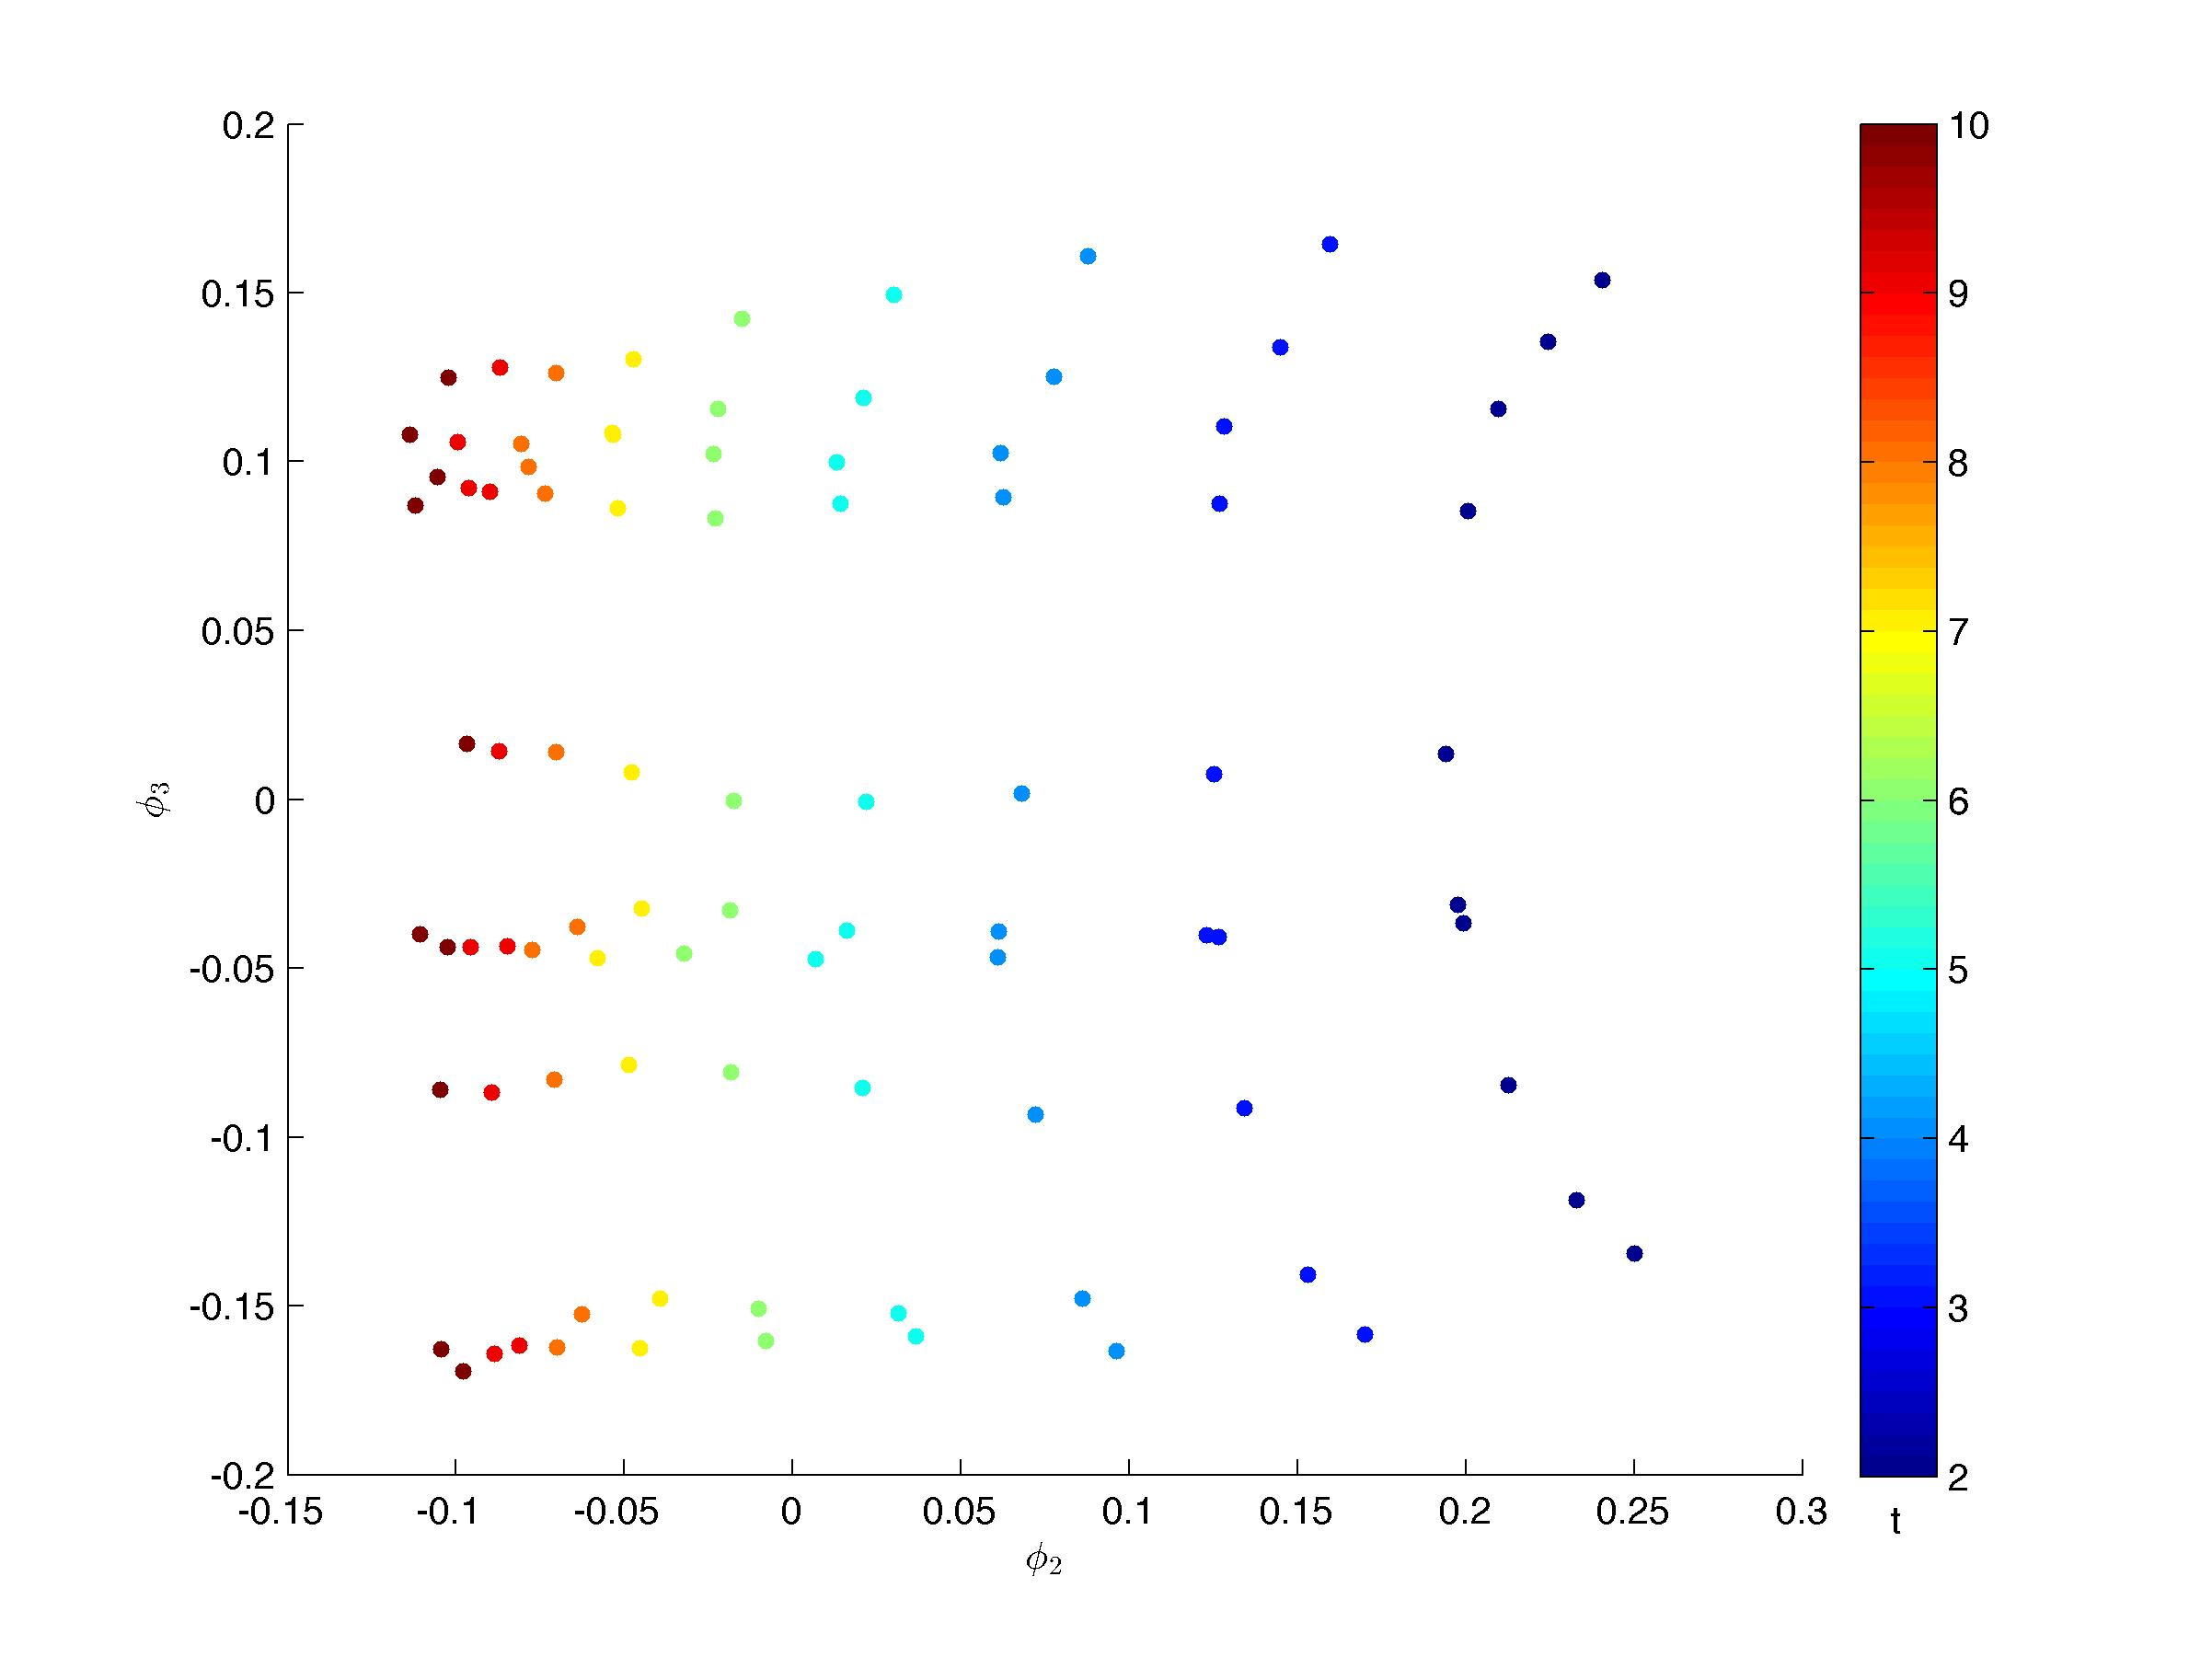
\includegraphics[width=\textwidth]{EMD_t_400}
\caption{}
\end{subfigure}
\caption{Diffusion maps embeddings computed from simulation data of the velocity jump process with (a,b) $\lambda=1$, $s=1$, and (c,d) $\lambda=400$, $s=20$. The distances used in the diffusion maps kernel are the earth mover's distances between the histograms of particle positions. The data are colored by (a, c) $p$, the initial probability of left--moving particles, and (b, d) $t$, time. One can see that these two parameters, $p$ and $t$, are well--correlated with the first two diffusion maps modes, $\phi_2$ and $\phi_3$. However, the ``more important'' mode, $\phi_2$, is correlated with $p$ for the small $\lambda$ case (a), and correalted with $t$ for the large $\lambda$ case (d). This is consistent with the asymptotic analysis discussed in Section \ref{subsec:mode_analysis}. In the small $\lambda$ regime (wave equation) in (a,b) we observe that for small time, the initial condition of the particle velocity does not play a significant role -- all the particles start at position $0$, and therefore, for small time, the particles are more condensed and it is more difficult to distinguish the particles moving to the left from the particles moving to the right. On the other hand, for large time, once the particles evolve from the origin, this separation is clear.  For the large $\lambda$ case (heat equation) in (c,d), we observe that for small time the initial distribution $p$ is well organized in the embedding (c), since for small time the distribution of the particles is skewed and the initial velocity plays a role in this regime. On the other hand, for large time, we observe that the initial distribution $p$ is not organized as well in the embedding (c), since the velocities have equilibrated and so the initial distribution is less detectable in the particle distribution.}
\label{fig:dmaps_embed}
\end{figure}

\section{Discussion}


\bibliography{references}

\end{document}